\documentclass[11pt,paper=letter]{scrartcl}
\usepackage[wide]{cjquines}

\newcommand{\btn}[1]{\;\boxed{#1}\;}

\begin{document}

\title{Four-Function Primality Testing}
\author{Carl Joshua Quines}
\date{August 13, 2019}

\maketitle

% \begin{abstract}
%   We set up a model of computation using a four-function calculator, and discuss several primality tests. Along the way, we'll talk about the algorithmic analysis and the distribution of primes.
% \end{abstract}

\noindent Here's a problem. Consider these three numbers:
$$5923,\quad 524\,717,\quad 123\,456\,789\,011.$$
You have the calculator in the following picture:
\begin{center}
  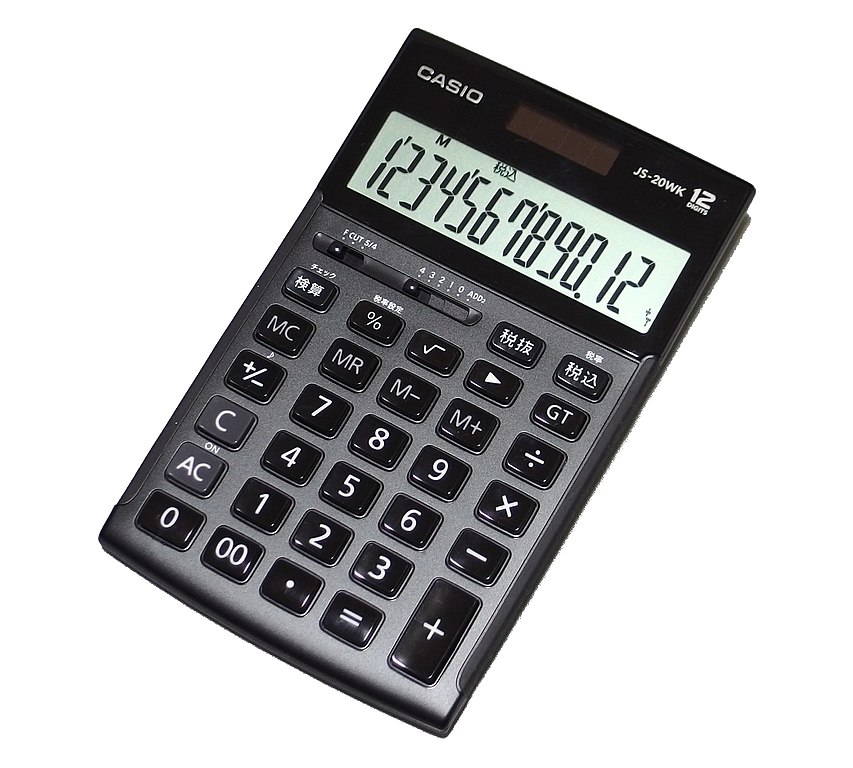
\includegraphics[height=2.5in]{1.jpg}
\end{center}
You also have a pen and paper. Using these tools, how long would it take you to check if each of these three numbers are prime? Make a quick guess. An all-nighter? A whole day? Even longer?

In fact, I claim it's possible to check if these three numbers are prime, in \textbf{twenty minutes} in total, and here I'll talk about how.

Note that the point of this handout isn't to present a feasible way to do primality testing by hand! If you wanted to check if these numbers are prime, I recommend looking them up in \href{https://www.wolframalpha.com/input/?i=is+123456789011+prime}{Wolfram Alpha}. Instead, the point of this handout is to discuss some \textbf{computational number theory}. We'll learn about algorithmic analysis, the Fermat and Miller--Rabin tests, binary exponentiation, and big integers.

\section{Trial division}

You might believe that this is feasible for $5923$. To check that it's prime, all we have to do is to check that no number smaller than it divides $5923$. So we divide $5923$ by $2$, and then we divide it by $3$, and then by $4$, and so on. If at any point we get an integer, we know it can't be a prime.

With this strategy, we need to check at most $5\,921$ numbers: $2$, $3$, $4$, and so on, up to $5\,922$. In the worst-case when the number \textbf{is} prime, then we have to check \textbf{all} numbers before we're sure it's prime. Even if we can type the numbers in the calculator quickly enough to do one division per second, it would still take about six thousand seconds, which is about 1 hour and 40 minutes.

Surely we can do faster! Instead of checking all the numbers up to $5\,921$, we in fact only need to check all the numbers up to $\sqrt{5923}$. This is because if there was a factor $d$ of it larger than the square root, then there's a factor smaller than the square root, which is $\frac{5923}{d}$. Our calculator has a square root button, so we check that $\sqrt{5923} = 76.96\ldots$, so we only need to check the numbers up to $76$.

This is definitely doable in under two minutes! By using the MR button, we don't even have to type $5923$ every time. We type $5923$ once and press M+. Then pressing MR will bring up the number $5923$. So the button presses look like MR, $\div$, $2$, MR, $\div$, $3$, and so on. Doing this, we see this number is actually prime.

For $524\,717$, however, its square root is about $724$. So with the one division per second estimate, it would take twelve minutes, which is a bit too long. But we don't have to check all $724$ numbers: we only need to check the primes. We don't have to check if it's divisible by $6$, because we already checked if it's divisible by $2$.

I magically know that there are $128$ primes less than $724$. If we had a list of these $128$ primes, then doing one division per second, it would take us a little more than two minutes to check, and that's fast enough for our purposes. Of course, we need a list of primes in the first place, which definitely will take more than two minutes to find.

But for the next number, $123\,456\,789\,011$, its square root is $351\,364$, and I magically know there are $30,084$ primes less than this. So this would definitely not be fast enough; even finding the primes would take a long time. We'll need to use a different strategy after this point.

\subsection{Analysis}

We've discussed three different strategies so far. Each of these strategies involve testing out possible factors using division, which is why we call these strategies \textbf{trial division}. If the number we're testing is $N$, then we have three strategies:
\begin{enumerate}[itemsep=-0.5ex]
  \item[S1.] Test all the numbers up to $N$.
  \item[S2.] Test all the numbers up to $\sqrt{N}$.
  \item[S3.] Test all the primes up to $\sqrt{N}$.
\end{enumerate}
S3 is a bit hard to do in practice, because we'd need to find a list of primes up to $\sqrt{N}$. For small $N$ this won't take that long to create ourselves, but when big $N$ this is a problem. In practice, most people do something in between S2 and S3: we test all numbers up to $\sqrt{N}$, skipping ones that are obviously composite, like ones divisible by $2$, $3$, or $5$. Let's call this strategy S2.5:
\begin{enumerate}
  \item[S2.5.] Test $2$, $3$, $5$, and all other numbers up to $\sqrt{N}$ that aren't divisible by $2$, $3$, or $5$.
\end{enumerate}
We can make a table counting the number of divisions, \textbf{in the worst-case}, that we have to do with each of these strategies. For example, for $N = 100$, we only have to do one division. But if we didn't know that, and we were using Strategy 1, then in the worst case, we do $98$ divisions.

Here's a table of the worst-case numbers of divisions for $N$ from a hundred to a billion. I've also indicated the time this takes. For the rest of the paper, we'll make the assumption that we can do \textbf{one calculator operation per second}. This gives these times:
\begin{center}
\begin{tabular}{rrlrlrl}
$N$                & S1    & Time     & S2 & Time     & S2.5 & Time     \\ \hline
100              & 98            & 2 mins.  & 9          & 9 secs.  & 5          & 5 secs.  \\
1\,000           & 998           & 16 mins. & 30         & 30 secs. & 11         & 11 secs. \\
10\,000          & 9\,998        & 3 hours  & 99         & 3 mins.  & 29         & 29 secs. \\
100\,000         & 99\,998       & 1 day    & 315        & 5 mins.  & 87         & 1 min.   \\
1\,000\,000      & 999\,998      & 11 days  & 999        & 16 mins. & 269        & 4 mins.  \\
10\,000\,000     & 9\,999\,998   & 3 months & 3\,161     & 52 mins. & 846        & 14 mins.  \\
100\,000\,000    & 99\,999\,998  & 3 years  & 9\,999     & 3 hours  & 2\,669     & 44 mins. \\
1\,000\,000\,000 & 999\,999\,998 & 32 years & 31\,621    & 9 hours  & 8\,436     & 2 hours
\end{tabular}
\end{center}

So we can see that S1 is very slow! If the number is $N$, it takes about $N$ seconds to compute. S2 takes about $\sqrt{N}$ seconds, which still takes a pretty long time, and S2.5, we can see, looks like it's about $\frac14\sqrt{N}$ seconds.

How fast is S2.5, exactly? Well, about half of the integers are odd, and two-thirds of those aren't divisible by three, and four-fifths of those aren't divisible by five. So the fraction of integers not divisible by $2$, $3$, or $5$ is $\frac12 \times \frac23 \times \frac45 = \frac8{30}$. So we're testing around $\frac8{30}\sqrt{N} + 3$ numbers.

This is the essence of something computer scientists call \textbf{algorithmic analysis}. In computer science, we call our strategies \textbf{algorithms} instead, and we're analyzing how long each algorithm would take depending on the size of the input. In typical analysis, we usually treat a single operation, like an addition, subtraction, multiplication or division, as a single time step, and then analyze how long it takes as a function of $N$.

One important idea in analyzing algorithms is something called \textbf{big O notation}. Let's go back: S1 takes around $N$ steps, S2 takes around $\sqrt{N}$ steps, and S2.5 takes around $\frac8{30}\sqrt{N} + 3$ steps. When we take the big O notation, we ignore the constants. So we say that S1 is $O(N)$, S2 is $O(\sqrt{N})$, and S2.5 is also $O(\sqrt{N})$.

Why is it okay for us to ignore the constants? Sure, S2.5 is faster than S2, but only four times faster, what we call a \textbf{constant improvement}. Most of the time, constant improvement isn't that hard to achieve. If we wanted to make S2 four times faster, we can just add more people. Four people doing S2 takes about the same time as one person doing S2.5, no matter how large $N$ is.

On the other hand, the difference between S1 and S2 is genuinely different. A single person doing S2 beats $10$ people doing S1 for $N > 100$. A single person doing S2 beats $100$ people doing S1 for $N > 10\,000$. A single person doing S2 can even beat $1\,000$ people doing S1 for $N > 1\,000\,000$!

\begin{center}
  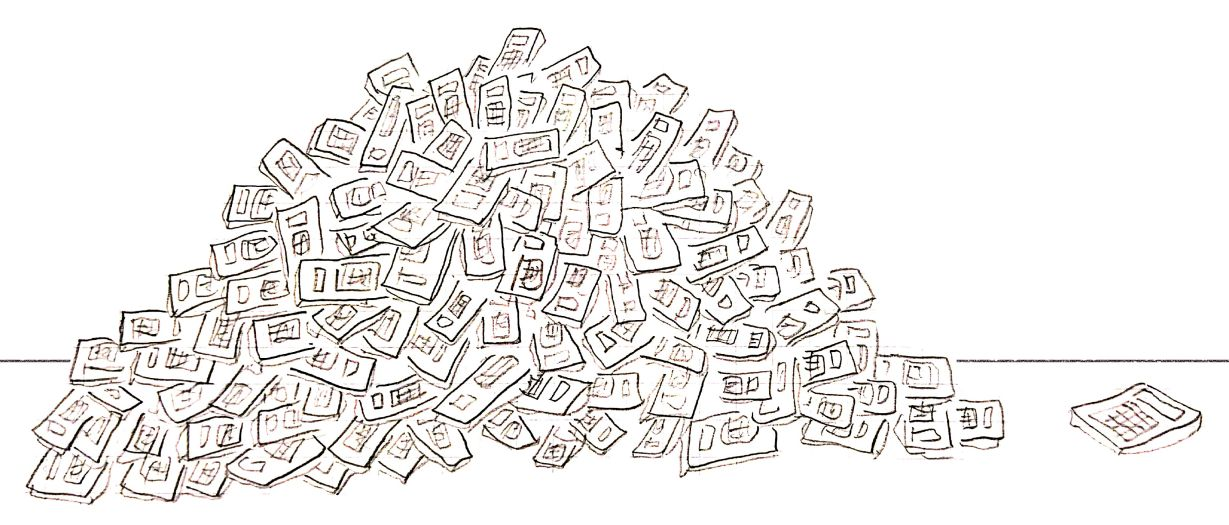
\includegraphics[height=2.25in]{2.jpg}

  \emph{\footnotesize It doesn't matter how many calculators you have: a faster algorithm will win.}
\end{center}

It doesn't matter how many people you have doing S1, or how much constant improvement you can do to S1: for large enough $N$, S2 will certainly be faster.

Computer scientists love big O notation because it's a quick way to state this. It's also why people care about improving algorithms in terms of big O, rather than just constant improvement, because for large enough $N$, it's often the deciding factor.

\section{Fermat test}

Can we go faster than $O(\sqrt{N})$, then? In fact, we can, using something called the Fermat test. Recall that \textbf{Fermat's little theorem} says that if $p$ is a prime, then $a^{p-1} \equiv 1 \pmod p$ when $a \not\equiv 0 \pmod p$. So if a number $p$ is prime, then this congruence should be true for any $a$ that we pick.

Now let $N$ be any integer, and let $a \not\equiv 0 \pmod N$. If $a^{N-1} \not\equiv 1 \pmod N$, then we're guaranteed that $N$ can't be prime. (Because otherwise, it would be equal to $1$.) We call $a$ a \textbf{witness} that $N$ is composite. And sometimes it is equal to $1$, in which case we call $a$ a \textbf{liar}, like it's misleading us to think that $N$ is prime.

It turns out that, for ``most'' numbers, there are few liars and more witnesses. For example, take $m = 15$. When $a \equiv 1$ or $a \equiv -1$, then $a^{14} \equiv 1$, and we know in advance that these will be liars. Ignoring these liars, there are only two other liars, which are $4$ and $11$:

\begin{center}
  \begin{tabular}{c|cccccccccccccc}
  $a$ & 1 & 2 & 3 & \textbf{4} & 5 & 6 & 7 & 8 & 9 & 10 & \textbf{11} & 12 & 13 & 14 \\ \hline
  $a^{14}\bmod 15$ & 1 & 4 & 9 & \textbf{1} & 10 & 6 & 4 & 4 & 6 & 10 & \textbf{1} & 9 & 4 & 1
  \end{tabular}
\end{center}

Here's the same thing for $m = 21$, where there are also only two non-obvious liars:

\begin{center}
  \begin{tabular}{c|cccccccccccccccc}
  $a$ & 1 & 2 & 3 & 4 & 5 & 6 & 7 & \textbf{8} & 9 & 10 & 11 & 12 & \textbf{13} & 14 & 15 & $\cdots$ \\ \hline
  $a^{20}\bmod 21$ & 1 & 4 & 9 & 16 & 4 & 15 & 7 & \textbf{1} & 18 & 16 & 16 & 18 & \textbf{1} & 7 & 15 & $\cdots$
  \end{tabular}
\end{center}

On the other hand, for an actual prime, \textbf{all} of the numbers will be $1$:

\begin{center}
  \begin{tabular}{c|cccccccccccccccc}
  $a$ & 1 & 2 & 3 & 4 & 5 & 6 & 7 & 8 & 9 & 10 & 11 & 12 & 13 & 14 & 15 & 16 \\ \hline
  $a^{16}\bmod 17$ & 1 & 1 & 1 & 1 & 1 & 1 & 1 & 1 & 1 & 1 & 1 & 1 & 1 & 1 & 1 & 1
  \end{tabular}
\end{center}

So this is the \textbf{Fermat test}. We pick a number $a$ that isn't $1$ or $N-1$, raise it to the power $N - 1$, and then check if it's $1$ modulo $N$. If it isn't, we know it's definitely composite. If it is, then we \textbf{guess} that it's prime---it's not assured, but it should be somewhat likely. If we want to be more sure, we can run the Fermat test several times with other choices of $a$ until we're sure enough.

As an example, take $1105$. We pick $2$. Then $2^{1104} \equiv 1 \pmod{1105}$, through some computation we'll talk about later. So it's looking like it'll be a prime, but let's try a few more just to be safe. If we pick $3$, then $3^{1\,104} \equiv 1 \pmod{1105}$, looking good. But then if we pick $5$, then $5^{1\,104} \equiv 885 \pmod{1105}$. So $5$ is a witness that $1105$ is composite, and $2$ and $3$ were actually liars.

\subsection{Probabilistic arguments}

In fact, if there is a witness to a number $N$ that's relatively prime to it, then it can be proven that more than half of the choices for $a$ are witnesses as well. Here's a quick sketch of the proof. Let $w$ be a witness. So $w^{N-1} \not \equiv 1 \pmod{N}$. Similarly, if $\ell$ is a liar, then $\ell^{N-1} \equiv 1 \pmod{N}$. Observe that $w\ell$ is now a witness, because
$$\del{w\ell}^{N-1} \equiv w^{N-1} \ell^{N-1} \equiv w^{N-1} \not\equiv 1 \pmod{N}.$$
So if you multiply $w$ by a liar, you get a witness. And if you multiply by a different liar, you get a different witness.\footnote{This is where we use the fact that $w$ is relatively prime to $N$. Suppose two products are the same, like $w\ell \equiv w\ell' \pmod N$. Then we can cancel by $w$ because it's relatively prime to $N$. Thus $\ell \equiv \ell' \pmod N$ and they are actually the same liar, not different liars.} So each liar, multiplied to $w$, gives us a different witness. Therefore, the number of witnesses is at least the number of liars! And since each number up to $N$ is either a liar or a witness, the number of witnesses is at least half of $N$.

So if there does exist a relatively prime witness, then we can be very confident that $N$ is prime after trying sufficiently many numbers. In this case, if we picked $a$ randomly, the probability it's a liar is less than $\frac12$. If we ran the test ten times, the probability we get a liar \textbf{every time} is $\del{\frac12}^{10}$, which is incredibly small. It's way more likely that one of our random choices gives us a witness.

\begin{center}
  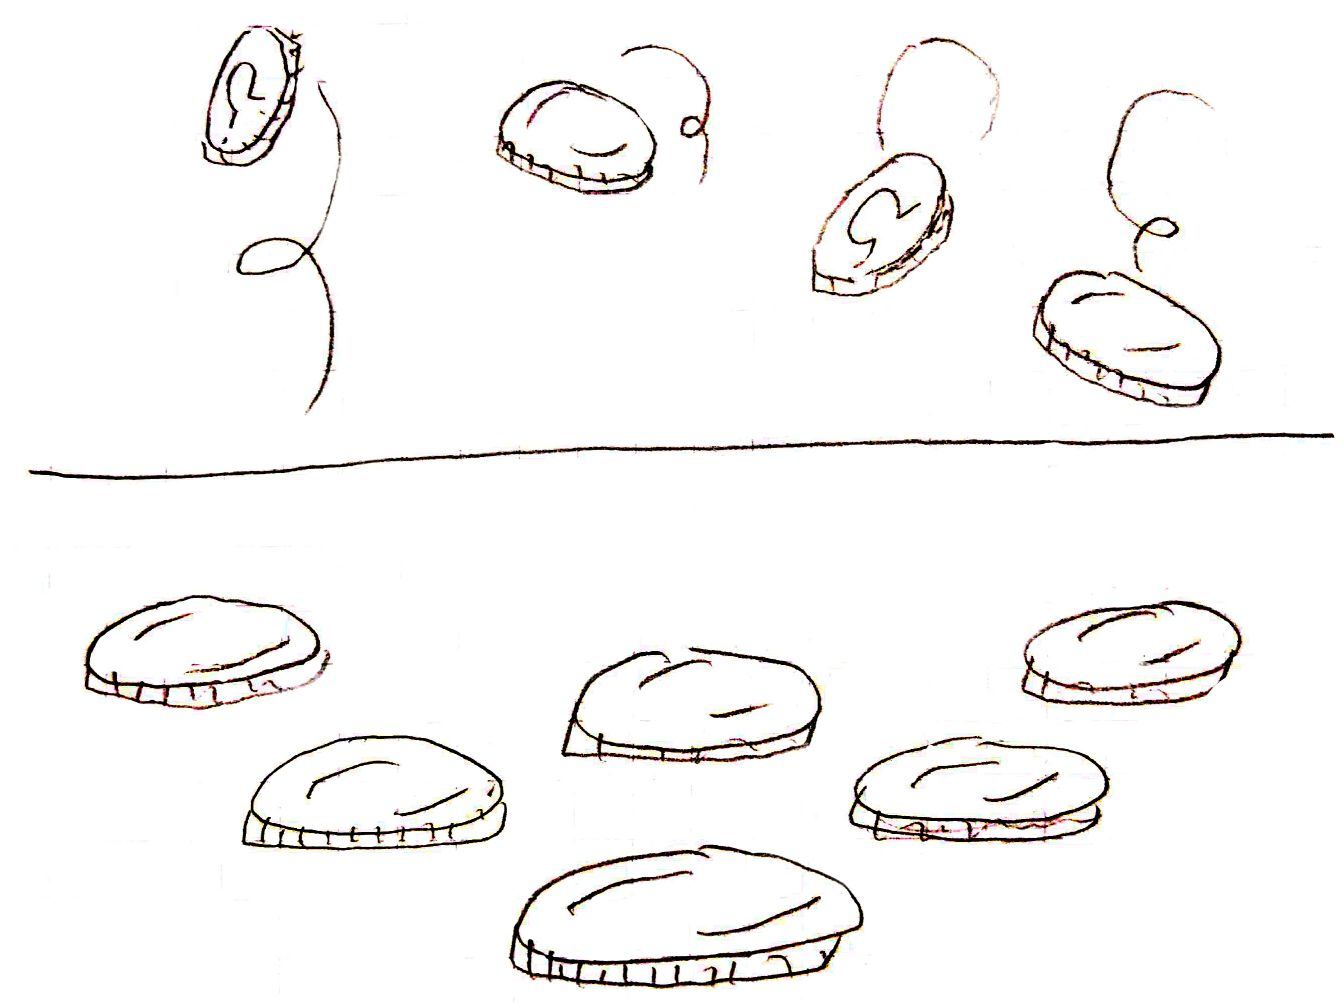
\includegraphics[height=2in]{3.jpg}

  \emph{\footnotesize It's more likely to flip ten coins and get tails each time.}
\end{center}

However, these arguments apply only if a relatively prime witness exists in the first place. In fact, there are some bad numbers where none of these exist, and there are fewer witnesses. Worse, there are numbers where \textbf{no} witnesses exist, and all of the choices are actually liars!

An example of such a number is $561$, where we claim that $a^{560} \equiv 1 \pmod{561}$ for all $a \neq 0$. We can factor $561 = 3 \times 11 \times 17$, so by the Chinese remainder theorem, we only need to show that
$$a^{560} \equiv 1 \pmod{3}, \qquad a^{560} \equiv 1 \pmod{11}, \qquad a^{560} \equiv 1 \pmod{17}.$$
But each of these are true by Fermat's little theorem. For example, for $11$, we have
$$a^{560} \equiv \del{a^{10}}^{56} \equiv 1^{56} \equiv 1 \pmod{11},$$
and we can check that something similar works for $3$ and $17$. Such numbers where all the choices are liars are called \textbf{Carmichael numbers}, and the Fermat test can't distinguish between primes and Carmichael numbers.

\subsection{Doing modulo quickly}

Suppose we were satisfied with this. After running the Fermat test on $N$ like ten times, we'd be reasonably confident that $N$ is either a prime or a Carmichael number. How fast can we compute this on a four-function calculator?

Let's recap the steps of the Fermat test. We have a number $N$ that we want to check is a prime or Carmichael number. Then we:
\begin{enumerate}
  \item Pick a random number $1 < a < N - 1$.
  \item Find $a^{N-1} \bmod N$.
  \item If we don't get $1$, we say $N$ is \textbf{composite}.
  \item Otherwise, we repeat the test, say around ten times. If we get $1$s every time, it's \textbf{maybe prime} or a \textbf{Carmichael} number.
\end{enumerate}
How quickly can we do a single test on a calculator? The main problem is computing $a^{N-1}$ modulo $N$. For most $N$, the problem is even getting it to fit in the calculator in the first place! Even for something as small as $N = 47$, $2^{46}$ is already too big to fit in our twelve-digit calculator.

The first trick is that we have to \textbf{reduce modulo $N$} every time we multiply. So for example, suppose we pick $2$. Then we multiply it by itself until we get $2^{39} = 549\,755\,813\,888$, which is twelve digits. If we multiply by $2$ again, it won't fit on the calculator anymore.

So we instead take it modulo $N$. The result will have to be smaller than $N$, and if $N$ is less than twelve digits, we can multiply by $2$ again and it'll fit. Every time we're going to hit something that doesn't fit, we take modulo $N$ before continuing.

Unfortunately, our calculator does not have a modulo function, so we'll have to figure out how to do modulo quickly. We can use the memory to reduce the number of button presses we have to use:

% \begin{enumerate}
%   \item Begin with $a$ on the calculator. Press MC to clear the memory, then M+, changing the memory to $a$.
%   \item Divide by $N$. Press $\blacktriangleright$ repeatedly until the decimals are gone, giving $\floor{\frac{a}{N}}$.
%   \item Multiply by $N$, giving $\floor{\frac{a}{N}}N$.
%   \item Then press M$-$, which subtracts the display from the memory, changing the memory to $a - \floor{\frac{a}{N}}N$.
%   \item Press MR to bring up the memory, which is $a \bmod N$.
% \end{enumerate}

% This one requires typing in $N$ twice, but it doesn't rely on the memory being anything specific in the beginning. An alternative doesn't require us to type in $N$ every time, but it restricts us to keeping $N$ in memory all throughout:

\begin{enumerate}
  \item Load $N$ in memory. (Press MC to clear the memory, type $N$, press M+.) For the rest of the calculation, the memory will always store $M$.
  \item Begin with $a$ on the calculator. Write it down on the sheet of paper.
  \item Divide by $N$ by pressing $\div$, then MR, then $=$. Press $\blacktriangleright$ repeatedly until the decimals are gone, giving $\floor{\frac{a}{N}}$.
  \item Multiply by $N$ by pressing $\times$, then MR, then $=$, giving $\floor{\frac{a}{N}}N$.
  \item Press $\pm$ to switch the sign. Then add $a$, written down earlier, to get $a - \floor{\frac{a}{N}}N$, which is $a \bmod N$.
\end{enumerate}

% illustration: calculator

% This second method requires writing down $a$ then typing it in again, which can be substantially slower. However, it also has the advantage of storing $a$ on the sheet of paper, which may be helpful if we need this result later.

% Either way, we have a relatively fast way of finding something modulo $N$. But the problem is, we'd need to multiply $a$ by itself $N-1$ times in order to find $a^{N-1} \bmod N$. In other words, this algorithm is $O(N)$. This is slower than trial division, which we know to be $O(\sqrt{N})$.

So we have a fast way of finding something modulo $N$, which takes around three seconds. The real bottleneck here is how fast you can write down $a$ on the sheet of paper, so you'd have to learn to write numbers quickly.

We still have a different problem. We'd need to multiply $a$ by itself $N-1$ times in order to find $a^{N-1} \bmod N$. So finding this would still take $O(N)$. This is slower than trial division, which we know to be $O(\sqrt{N})$.

\subsection{Exponentiating quickly}

But can we go faster? The problem of computing $a^{\text{something}} \bmod N$ is known as \textbf{modular exponentiation}. The second trick is that we can actually solve this problem in $O(\log_2 N)$ using an algorithm called \textbf{binary exponentiation}.

As the name suggests, it involves using binary. We can represent any number, like $37$, as a sum of powers of two, its \textbf{binary representation}. So $37 = 32 + 4 + 1$. And the idea is, we can find $a^{37}$ by multiplying $a^{32}$, $a^{4}$, and $a^1$. So we would only need to find $a$ rasied to powers of two, which we can do through repeated squaring.

Here's an example. Let's say we're computing $13^{81} \bmod 1000$. Then we compute $13^2 \equiv \mathbf{169} \pmod{1000}$. Then:
\begin{align*}
  13^4 \equiv \del{13^2}^2 \equiv (169)^2 &\equiv \phantom{0}28\,\mathbf{561}, \pmod{1000} \\
  13^8 \equiv \del{13^4}^2 \equiv (561)^2 &\equiv 314\,\mathbf{721}, \pmod{1000} \\
  13^{16} \equiv \del{13^8}^2 \equiv (721)^2 &\equiv 519\,\mathbf{841}. \pmod{1000}
\end{align*}
We can continue this way to fill up the following table:
\begin{center}
  \begin{tabular}{c|ccccccc}
  $k$ & 1 & 2 & 4 & 8 & 16 & 32 & 64 \\ \hline
  $13^k \bmod 1000$ & 13 & 169 & 561 & 721 & 841 & 281 & 961
  \end{tabular}
\end{center}
Then
$$13^{81} \equiv 13^{64} \times 13^{16} \times 13^1 \equiv 961 \times 841 \times 13 \equiv 613 \pmod{1000}.$$
And the advantage of our previous method of taking modulo $N$, which requires writing $a$ on a sheet of paper, can now be used to our advantage! Let $2^k$ be the largest power of two that is at most $N-1$. Then our new method for finding $a^{N-1} \bmod N$ is now:
\begin{enumerate}
  \item Compute $a^2 \bmod N$. While taking modulo $N$, we write the result down.
  \item Compute $a^4 = (a^2)^2 \bmod N$; note that we also write it down.
  \item Compute $a^8 = (a^4)^2 \bmod N$, which we also write down.
  \item And so on until $a^{2^k} = \del{a^{2^{k-1}}}^2 \bmod N$, all of which we write down.
  \item Then express $N-1$ in binary. We've conveniently written down the values of $a^{2^i} \bmod N$ earlier, so we can use these and the method shown previously, to find $a^{N-1} \bmod N$.
\end{enumerate}

\subsection{An example}

Let's run a Fermat test with our four-function calculator, using $524\,717$ as $N$. We start by clearing the memory by pressing MC, then type $524\,717$, then M+ to load it into memory.

Then we convert $N-1$ to binary. Since $524\,717$ is already on my screen, I subtract $1$ to get $524\,716$. Then I press $\div$, then $2$ to get $262\,358$. No remainder, so the last digit is a $0$. I divide by two again to get $131\,179$, no remainder, so the second-to-last digit is also $0$. Then I divide by two again to get $65\,589.5$, which has a remainder, so the next digit is $1$. Then I press $\blacktriangleright$ to remove the $.5$ before dividing by two again. The process of converting to binary is shown in the following table:
\begin{center}
  \begin{tabular}{ccccccccc}
    $262\,358$ & $131\,179$ & $65\,589.5$  & $32\,794.5$  & $16\,397$  & $8198.5$   & $4099$   & $2049.5$ & $1024.5$ \\ \hline
    0 & 0 & 1 & 1 & 0 & 1 & 0 & 1 & 1
  \end{tabular}
\end{center}
I then recognize that $1\,024$ is a power of two! So conveniently enough, the rest of the right column will be ten $0$s followed by a $1$, without having to do any more divisions.

On the sheet of paper, I only have the bottom row written, and it's written vertically, going downward. This is the binary expansion in reverse. The actual binary expansion is $524\,716 = 10\,000\,000\,000\,110\,101\,100_2,$ but the reverse binary expansion is actually more useful for us in this case.

Then we begin with the actual Fermat test. We'll pick $a = 2$. I write down $2$ below the first $0$ on my sheet of paper, then repeatedly square it. I don't actually have to take the modulo until it overflows. My sheet of paper now looks like:
\begin{center}
  \begin{tabular}{rr}
    0 & 2 \\
    0 & 4 \\
    \textbf{1} & \textbf{16} \\
    \textbf{1} & \textbf{256} \\
    0 & 65\,536 \\
    1 & \\
    $\vdots$ & $\vdots$
  \end{tabular}
\end{center}
I can't square $65\,536$ in my head, so I turn to the calculator. I type in $65\,536$, hit $\times$, type in $65\,536$, then do the steps to take the modulo. I get $158\,651$. So I write this down underneath the next column, and I repeat this process about fourteen more times to fill in the rest of the table:
\begin{center}
  \begin{tabular}{rrcrr}
    $\vdots$ & $\vdots$ & $\phantom{a\quad a}$ & $\vdots$ & $\vdots$ \\
    0 &  65\,536 & & 0 & 274\,380 \\
    \textbf{1} & \textbf{158\,651} & & 0 &  88\,108 \\
    0 & 514\,745 & & 0 & 365\,366 \\
    \textbf{1} & \textbf{269\,271} & & 0 & 519\,880 \\
    \textbf{1} & \textbf{426\,947} & & 0 & 309\,021 \\
    0 & 203\,311 & & 0 & 206\,894 \\
    0 & 256\,329 & & 0 & 288\,527 \\
    0 &  18\,218 & & \textbf{1} & \textbf{428\,245} \\
    $\vdots$ & $\vdots$ & & &
  \end{tabular}
\end{center}
And now the reverse binary expansion becomes helpful, because to find the value of $2^{524\,716} \bmod 524\,717$, I'll multiply all the entries corresponding to $1$s:
$$16 \times 256 \times 158\,651 \times 269\,271 \times 426\,947 \times 428\,245 = 240\,181.$$
So $2^{524\,716} \equiv 240\,181 \pmod{524\,717}$. It's not $1$, and thus $2$ is a witness that \textbf{524\,717 is composite}, and we don't need to run any more tests. In fact, $524\,717 = 647 \times 811$, so trial division would take a long time before finding out that this number is composite. On the other hand, a single Fermat test showed us this.

\subsection{Analysis}

How long does a Fermat test take? The slow part is squaring and then taking modulo $N$ for $k$ times, where $2^k$ is the largest power of two less than $N$. Each time we square and modulo $N$ takes only a few seconds, if we write fast enough. And the number of times we do this is $k$. Since $2^k < N$, we get $k < \log_2 N$. Ignoring the constants, like we always do for big O notation, this algorithm is $O(\log_2 N)$.

How fast is this? Well, for $524\,717$, $k$ is $18$. Running the Fermat test once would take around a minute and a half, by our standard of one operation per second. So running ten of them would take around fifteen minutes. The great thing about this is that even for large numbers like $123\,456\,789\,011$, $k$ is still $36$. Even if the number became a million times bigger, $k$ only doubled!

Using this estimate, here's a table showing how long it would take to run ten Fermat tests on a number of about size $N$, compared to our trial division strategies from earlier:
\begin{center}
\begin{tabular}{rllll}
$N$              & S1       & S2       & S2.5     & 10$\times$ Fermat \\ \hline
100              & 2 mins.  & 9 secs.  & 5 secs.  & 5 mins. \\
1\,000           & 16 mins. & 30 secs. & 11 secs. & 7 mins. \\
10\,000          & 3 hours  & 3 mins.  & 29 secs. & 10 mins. \\
100\,000         & 1 day    & 5 mins.  & 1 min.   & 13 mins. \\
1\,000\,000      & 11 days  & 16 mins. & 4 mins.  & 15 mins. \\
10\,000\,000     & 3 months & 52 mins. & 14 mins. & 19 mins. \\
100\,000\,000    & 3 years  & 3 hours  & 44 mins. & 21 mins. \\
1\,000\,000\,000 & 32 years & 9 hours  & 2 hours  & 24 mins.
\end{tabular}
\end{center}
Even if ten Fermat tests is slower for smaller numbers, we see that it's actually \textbf{better} for larger numbers! This is the idea we've been talking about earlier: a strategy that's $O(\log_2 N)$ will \textbf{always} beat any $O(\sqrt N)$ strategy, when $N$ is large enough.

The $O(\sqrt N)$ strategy might be better for small $N$, like we see here. But as $N$ grows larger, we need to start worrying about our strategy and how fast it is.

\section{Miller--Rabin test}

The Fermat test is good, but it's not the best test. It can't tell the difference between primes and Carmichael numbers, and there are certain really bad prime numbers that have lots of liars. There's an improvement called the \textbf{Miller--Rabin test} which is based on the Fermat test.

If a number $p$ is prime, how many solutions are there to $x^2 \equiv 1 \pmod p$? From the onset, we see there are two solutions, $-1$ and $1$, but are there more? In fact, modulo $p$, a polynomial of degree $d$ can only have at most $d$ roots, a result known as \textbf{Lagrange's theorem}. In this particular case, we can factor it as $$x^2 - 1 \equiv (x - 1)(x + 1) \pmod p \implies p \mid (x - 1)(x + 1),$$
and as $p$ is a prime, either $p \mid x - 1$ or $p \mid x + 1$. This means $x$ can only be $-1$ or $1$ modulo $p$. In other words, the \textbf{square root} of $1$, when $N$ is a prime, is $1$ or $-1$.

But when about the non-prime case? Say $x^2 \equiv 1 \pmod{105}$. By the Chinese remainder theorem, this is equivalent to solving
$$x^2 \equiv 1 \pmod 3, \qquad x^2 \equiv 1 \pmod 5, \qquad x^2 \equiv 1 \pmod 7.$$
Since each individual congruence has two solutions, the original must have $2 \times 2 \times 2 = 8$ different solutions modulo $105$. So if $x^2 \equiv 1 \pmod N$ has solutions other than $-1$ and $1$, we're \textbf{guaranteed} that $N$ is composite.

And the way to find such solutions is to go back to the Fermat test. Recall that we call $a$ a liar if $a^{N-1} \equiv 1 \pmod N$. In this case, we're not sure if $N$ is a prime or not. But if $N$ was a prime, then by the previous remark, $a^{\frac{N-1}2} \equiv -1 \text{ or } 1 \pmod N$. If it wasn't, then we would be guaranteed that $N$ is composite!

Let's see this for $N = 15$. We earlier saw that there were two liars other than $-1$ and $1$, which are $4$ and $11$. That is, $4^{14} \equiv 11^{14} \equiv 1 \pmod {15}$. But what happens if we look at $4^7$ or $11^7$?
\begin{center}
  \begin{tabular}{c|cccccccccccccc}
  $a$ & 1 & 2 & 3 & \textbf{4} & 5 & 6 & 7 & 8 & 9 & 10 & \textbf{11} & 12 & 13 & 14 \\ \hline
  $a^{14}\bmod 15$ & 1 & 4 & 9 & \textbf{1} & 10 & 6 & 4 & 4 & 6 & 10 & \textbf{1} & 9 & 4 & 1 \\
  $a^{7}\bmod 15$ & 1 & 8 & 12 & \textbf{4} & 5 & 6 & 13 & 2 & 9 & 10 & \textbf{11} & 3 & 7 & 14
  \end{tabular}
\end{center}
Miraculously, they're not $-1$ or $1$! So $4$ and $11$ are now \textbf{witnesses} that $15$ is composite! What about for $21$, where we had the liars $8$ and $13$? What are $8^{10} \bmod 21$ and $13^{10} \bmod 21$?
\begin{center}
  \begin{tabular}{c|cccccccccccccccc}
  $a$ & 1 & 2 & 3 & 4 & 5 & 6 & 7 & \textbf{8} & 9 & 10 & 11 & 12 & \textbf{13} & 14 & 15 & $\cdots$ \\ \hline
  $a^{20}\bmod 21$ & 1 & 4 & 9 & 16 & 4 & 15 & 7 & \textbf{1} & 18 & 16 & 16 & 18 & \textbf{1} & 7 & 15 & $\cdots$ \\
  $a^{10}\bmod 21$ & 1 & 16 & 18 & 4 & 16 & 15 & 7 & \textbf{1} & 9 & 4 & 4 & 19 & \textbf{1} & 7 & 15 & $\cdots$
  \end{tabular}
\end{center}
So that didn't work; we see that $8$ and $13$ are still liars. But we can apply the same argument again: if $a^{\frac{N-1}2} \equiv 1 \pmod N$, then we can check $a^{\frac{N-1}4} \bmod N$. If $N$ was a prime, it would be $-1$ or $1$, but if not, we know it's composite. Let's see:
\begin{center}
  \begin{tabular}{c|cccccccccccccccc}
  $a$ & 1 & 2 & 3 & 4 & 5 & 6 & 7 & \textbf{8} & 9 & 10 & 11 & 12 & \textbf{13} & 14 & 15 & $\cdots$ \\ \hline
  $a^{20}\bmod 21$ & 1 & 4 & 9 & 16 & 4 & 15 & 7 & \textbf{1} & 18 & 16 & 16 & 18 & \textbf{1} & 7 & 15 & $\cdots$ \\
  $a^{10}\bmod 21$ & 1 & 16 & 18 & 4 & 16 & 15 & 7 & \textbf{1} & 9 & 4 & 4 & 19 & \textbf{1} & 7 & 15 & $\cdots$ \\
  $a^{5}\bmod 21$ & 1 & 11 & 12 & 16 & 17 & 6 & 7 & \textbf{8} & 18 & 19 & 2 & 13 & \textbf{13} & 14 & 15 & $\cdots$
  \end{tabular}
\end{center}
Aha! Now $8$ and $13$ are witnesses that $21$ is composite too! In general, we can inspect $a^{N-1}, a^{\frac{N-1}2}, a^{\frac{N-1}{4}}$, and so on until we can't divide the exponent by $2$ any more.

Let's do another example, for $221$. Note that $174^{220} \equiv 1 \pmod{221}$. And also $174^{110} \equiv -1 \pmod{221}$. Then taking the square root another time won't tell us anything about $221$; we only know something about it when we're taking the square root of $x^2 \equiv 1 \pmod N$. So $174$ isn't a witness.

So let's try another base, like $103$. We compute that $103^{220} \equiv 1 \pmod{221}$. Then $103^{110} \equiv 1 \pmod{221}$ as well. But then $103^{55} \equiv 103 \pmod{221}$, so $103$ is a witness that $221$ is a composite number!

Let's summarize our current procedure. After picking a random $a$, neither equal to $1$ or $-1$, we then:

\begin{enumerate}
  \item Find the value of $a^{N-1} \bmod N$. If it's not $1$, $N$ is \textbf{composite}. Otherwise, we continue.
  \item Find the value of $a^{\frac{N-1}2} \bmod N$.
  \begin{itemize}
    \item If it's not $1$ or $-1$, $N$ is \textbf{composite}.
    \item If it's $-1$, there's no point to taking more square roots, so we stop and $N$ is \textbf{maybe prime}.
    \item Otherwise, it's $1$, and we take continue by taking the square root.
  \end{itemize}
  \item Find the value of $a^{\frac{N-1}4} \bmod N$.
  \begin{itemize}
    \item If it's not $1$ or $-1$, $N$ is \textbf{composite}.
    \item If it's $-1$, we stop and $N$ is \textbf{maybe prime}.
    \item Otherwise, we continue.
  \end{itemize}
  \item We keep going like this until we can't take square roots any more. If we didn't say $N$ is composite, we say $N$ is \textbf{maybe prime}.
\end{enumerate}

\subsection{Going backwards}

The \textbf{Miller--Rabin test} is this but done backwards. This is better so we don't have to do binary exponentiation with each of $N-1$, $\frac{N-1}2$, $\frac{N-1}4$, and so on.

So let's say that the most you can get by repeatedly halving $N-1$ is $d$. This means that $d$ is odd. Then let's write $N-1 = 2^r d$. Then the numbers we're looking at are
$$a^{d}, a^{2d}, a^{4d}, \ldots, a^{2^{r-2}d}, a^{2^{r-1}d}, a^{2^rd}.$$
(Note that this list of numbers is the same as
$$a^{\frac{N-1}{2^r}}, a^{\frac{N-1}{2^{r-1}}}, a^{\frac{N-1}{2^{r-2}}}, \ldots a^{\frac{N-1}{4}}, a^{\frac{N-1}{2}}, a^{N-1},$$
in that order.) What would this list look like if $N$ was a prime? Based on our previous procedure, we have two possible sequences. It would look like either
$$1, 1, 1, \ldots, 1,\quad\text{or}\quad \text{?}, \text{?}, \text{?}, \ldots, \text{?}, -1, 1, 1, 1, \ldots, 1,$$
where the question marks are some numbers. You should stop and check this: if we did the previous procedure on this sequence, we would say $N$ is maybe prime. Therefore, if we get anything other than this above sequence, we're now guaranteed that $N$ is composite! So the Miller--Rabin test is done as:
\begin{enumerate}
  \item Find the value of $a^{d} \bmod N$. If it's $1$, then we're going to get the first sequence above. We stop and say $N$ is \textbf{maybe prime}.
  \item Otherwise, find $a^{2d}, a^{4d}, \ldots, a^{2^{r-1}d}$, each modulo $N$. If any of these are $-1$, we're going to get the second sequence above. We stop and say $N$ is \textbf{maybe prime}.
  \item Otherwise, we're sure that $N$ is \textbf{composite}.
\end{enumerate}
As an exercise, think about why we don't need to check if $a^{2^rd}$ is $-1$. Like in the Fermat test, we call $a$ a \textbf{witness} for $N$ if it outputs composite for $N$, and a \textbf{liar} if it outputs maybe prime if $N$ is actually composite.

\subsection{Analysis}

How good is the Miller--Rabin test? Both the Fermat test and the Miller--Rabin test differ from trial division in that they're both \textbf{probabilistic}. That means that it doesn't guarantee us that a number is prime, but only tell us that there's a high probability it is a prime. So there's a chance that the test gives us a false positive.

Unlike the Fermat test, however, the Miller--Rabin test has better odds. It can be shown that for any composite $N$, at least $\frac34$ of the choices for $a$ are witnesses that it's composite. The argument is much more involved than the one for the Fermat test, so we won't go through it here.

Note, already, the difference here. Unlike the Fermat test, our guarantee doesn't rely a witness existing in the first place. It's true for \textbf{all} composite $N$, so there won't be any bad cases, like the Carmichael numbers. It's also a much better guarantee: running the test ten times gives a $\del{\frac14}^{10}$ chance of a false positive.

\begin{center}
  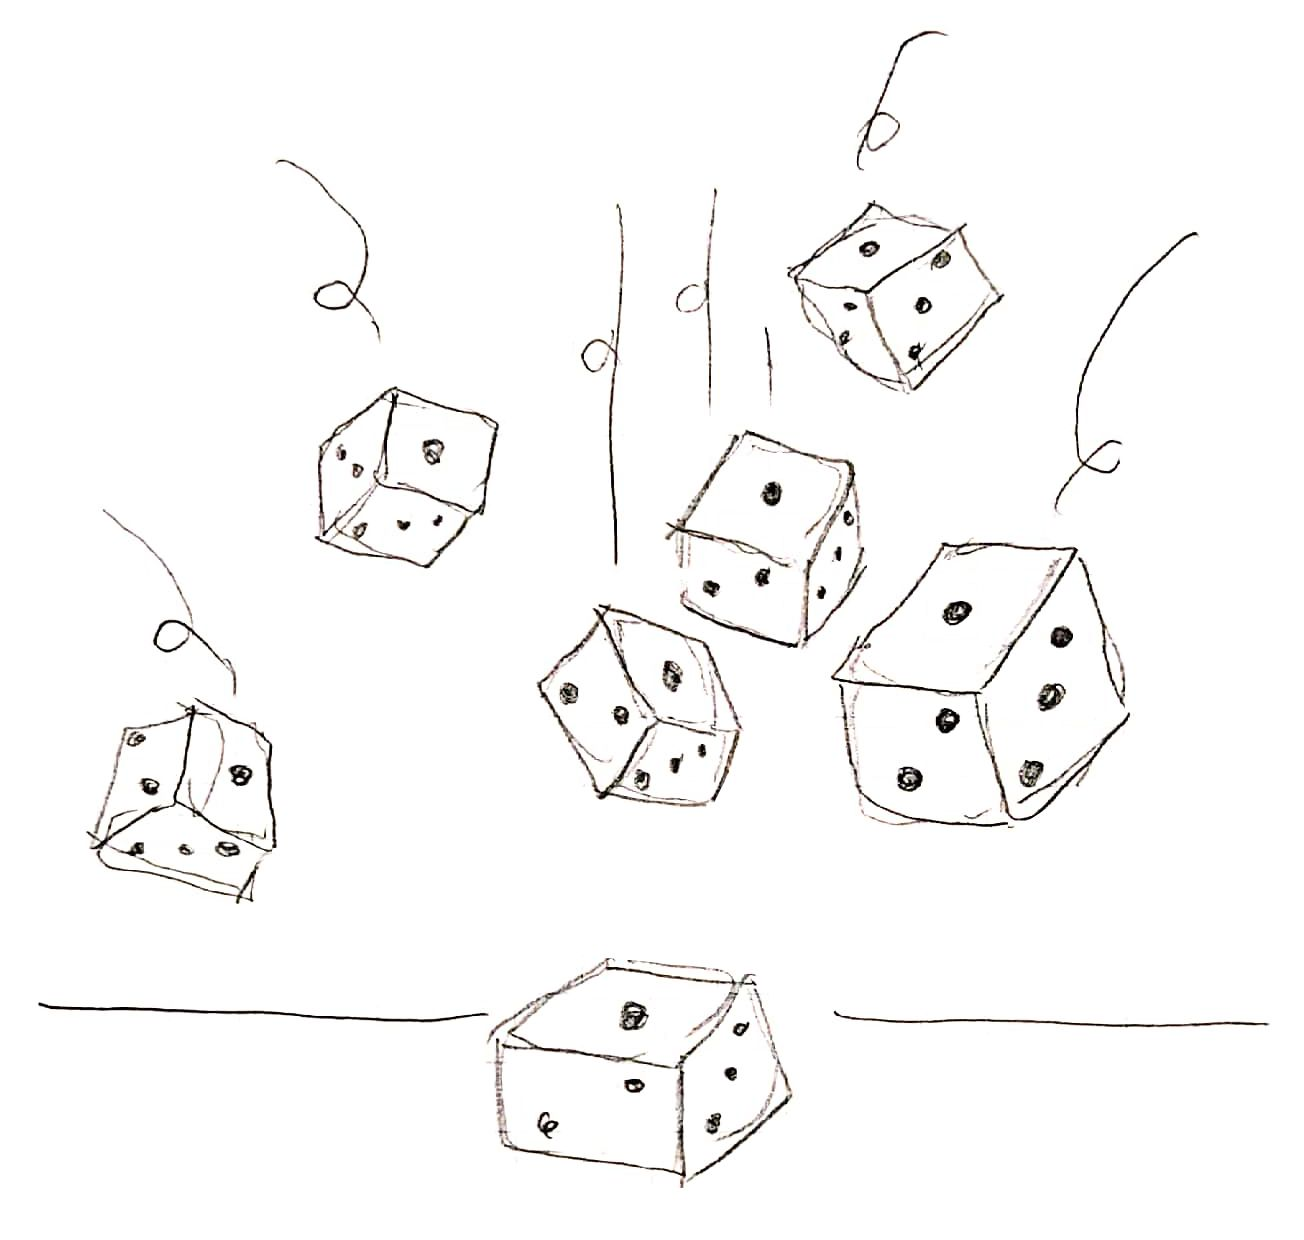
\includegraphics[height=2.25in]{4.jpg}

  \emph{\footnotesize It's more likely to roll seven dice and get one each time.}
\end{center}

In fact, when $N$ is small, computer searches have verified that a small set of $a$s serve as witnesses for all $N$ up to this size. For example, when $N < 1\,,373\,653$, then it's enough to test only $a = 2$ and $a = 3$! The fact that we only need to check two values of $a$ to verify everything up to a million should be very, very surprising, compared to our estimate of $\del{\frac14}^2$. This means that for most composite numbers, the number of liars is much less than $\frac14$ that number.

A good reference for small sets of numbers that verify everything is in \url{https://miller-rabin.appspot.com/}. The way to interpret this table is that the ``best solution'' column gives the largest $N$ it works for, and the bases is the set of $a$s you run Miller--Rabin on. For our purposes, there's a test that checks for all $N < 154\,639\,673\,381$, using only three $a$s:
$$15,\quad 176\,006\,322,\quad 4\,221\,622\,697.$$
An easier list to memorize would be: for everything up to ten digits, $2$, $7$, and $61$; for everything up to twelve digits, $2$, $3$, $5$, $7$, and $11$.

This is much better than doing the Fermat test, because we have a guarantee that it'll work for small numbers. It's faster too, since we have to run a Miller--Rabin test maybe twice or thrice, rather than ten times. Compare this to our previous tests:
\begin{center}
\begin{tabular}{rllllll}
$N$              & S1       & S2       & S2.5     & 10$\times$ Fermat & 2$\times$ MR & 3$\times$ MR \\ \hline
100              & 2 mins.  & 9 secs.  & 5 secs.  & 5 mins.  & 1 min.  & 1 min.  \\
1\,000           & 16 mins. & 30 secs. & 11 secs. & 7 mins.  & 1 min.  & 2 mins. \\
10\,000          & 3 hours  & 3 mins.  & 29 secs. & 10 mins. & 2 mins. & 3 mins. \\
100\,000         & 1 day    & 5 mins.  & 1 min.   & 13 mins. & 2 mins. & 4 mins. \\
1\,000\,000      & 11 days  & 16 mins. & 4 mins.  & 15 mins. & 3 mins. & 4 mins. \\
10\,000\,000     & 3 months & 52 mins. & 14 mins. & 19 mins. & ---     & 5 mins. \\
100\,000\,000    & 3 years  & 3 hours  & 44 mins. & 21 mins. & ---     & 6 mins. \\
1\,000\,000\,000 & 32 years & 9 hours  & 2 hours  & 24 mins. & ---     & 7 mins.
\end{tabular}
\end{center}
The 2$\times$ MR column shows how long it would take to do Miller--Rabin using $2$ and $3$, and the blank entries indicate that 2$\times$ MR isn't guaranteed to work for these numbers. The 3$\times$ MR column shows how long it would take to run it on $2$, $7$, and $61$.

We see that the improvement isn't spectacularly big. Both the Miller--Rabin test and the Fermat test are $O(\log_2 N)$, but the Miller--Rabin test is around three times faster for these numbers because we have to run it two or three times, instead of ten.

So we get a constant improvement doing the Miller--Rabin test over the Fermat test. But we still care about Miller--Rabin because it's more reliable than the Fermat test. The chance we get a false positive is smaller, and it works with Carmichael numbers. Another reason to care about it is because people have published short lists of witnesses that work for lots of numbers, which make it practically useful.

\subsection{Big integers}

To test that $N = 123\,456\,789\,011$ is prime, we know that we only need to run three Miller--Rabin tests. We've already discussed how to do modulo quickly, and there's no problem here. But if we try to do exponentiation, we quickly run into a problem: if $a$ is large, then $a^2$ won't fit in the calculator. Even if $a^2 \bmod N$ will fit in the calculator, $a^2$ will \textbf{overflow}---the answer will be too big to fit.

In particular, we need to figure out this problem: given $a$, which can be up to twelve digits long, how do we find $a^2 \bmod N$? We'll split this problem into two parts. First is finding $a^2$, then finding it mod $N$.

Finding $a^2$ is the less tedious part. We can split up $a$ as $10^6 \cdot b + c$, where both $b$ and $c$ have six digits. Then
$$ a^2 = \del{10^6 \cdot b + c}^2 = 10^{12} \cdot b^2 + 10^6 \cdot 2bc + c^2.$$
We can compute both $b^2$ and $c^2$ using the calculator. We can also compute $2bc$, but we have to be careful with overflow. If $bc$ happens to be larger than $5 \cdot 10^{11}$, then $2bc$ would overflow. The trick is to remove the last digit first by pressing $\blacktriangleright$. For example, to compute $878\,939\,830\,554 \times 2$, we do
$$878\,939\,830\,554 \btn{\blacktriangleright} 87\,893\,983\,055 \btn{\times} \btn{2} \btn{=} 175\,787\,966\,110,$$
and the final answer must be what we got, times ten, plus twice the removed digit. So the final answer is $1\,757\,879\,661\,108$. We can then add all the intermediate results $10^{12} \cdot b^2$, $10^6 \cdot 2bc$, and $c^2$, on paper. This is not too hard of a step; if you really wanted to, you can split the sum into twelve-digit parts which you can add with the calculator.

We now have the next part of the problem. We have some number $a^2$, possibly up to $24$ digits, and we need to find it modulo $N$. We're going to find it digit-by-digit, from left-to-right. We start with the first twelve digits, and find it mod $N$. Then at each step, we append the next digit, find it mod $N$ again, repeating until we're done.

For example, suppose our calculator had three digits instead of twelve, and we're finding a large number like $123\,456$ modulo $71$. What we do is:
\begin{itemize}[itemsep=-0.5ex]
  \item Find $123 \bmod 71$, which is $52$.
  \item We type the next digit, giving us $524$. Then we find $524 \bmod 71$, which is $27$.
  \item Type in $5$, getting $275$. Then $275 \bmod 71 = 62$.
  \item Finally, $626 \bmod 71 = 58$.
\end{itemize}
And indeed, we can check that $123\,456 \bmod 71 = 58$. To convince yourself this works, consider what it'd look like if you didn't take the modulo every time. Then you get the number itself. So intuitively, taking the modulo every time wouldn't change the final value. You can also try to show for yourself that this is true algebraically.

The trouble is that we might not be able to add in the next digit, since $N$ has twelve digits itself. When we take it modulo $N$, it's possible that we might end up with something a little larger than $10^{11}$, so we can't directly append the next digit.

To deal with this, suppose that the current number is $a$, and we want to append the digit $b$. In other words, we want to compute $(10a + b) \bmod N$. The trick is to compute $10a \bmod N$ as $2(5a \bmod N) \bmod N$. Then we can add $b$, and continue with the rest of the algorithm.

One final optimization we can make: the modulo operation we gave earlier is unnecessary in this case. Since the intermediate results are pretty close to $N$ anyway, it would be faster to just subtract $N$ repeatedly. We can hit $-$, then MR, then $=$. Then repeatedly pressing $=$ will repeat the previous operation, and we can eyeball when we're done. That way, our square and modulo operation would be much faster, since we don't have to write the number itself. This speeds it up to around ten seconds each time.

\subsection{As promised}

Time to deliver my promise. I claimed we could check if each of the three numbers in the introduction are prime in twenty minutes in total. So here:

\begin{itemize}
  \item For $5923$, we trial divide the primes until $\sqrt{5923} = 76$. It's not hard to memorize the primes up to this point. This takes around \textbf{20 seconds}.

  \item For $524\,717$, we do two Miller--Rabin tests. As $2^{19} > 524\,717$, converting to binary will take around 20 seconds, since we have to halve the number 19 times. In a single Miller--Rabin, we have to square and take the modulo 19 times as well, and in total that should take around 100 seconds. Doing this twice gives a little over \textbf{4 minutes}.

  \item For $123\,456\,789\,011$, we do three Miller--Rabin tests. Converting to binary would take around a minute, since we halve 36 times. In a single Miller--Rabin, we square and take the modulo 36 times as well. The square and modulo operation takes around 10 seconds. So a single Miller--Rabin takes 5 minutes. Doing this thrice gives \textbf{15 minutes}.
\end{itemize}

So our grand total is \textbf{20 minutes}; even if you add some margin, it'll take maybe half an hour. While there is no way I would actually want to try this out, this at least shows it's \emph{possible} to do this if you really had to. In the words of Henry Cohn, one of the \href{https://promys.org}{PROMYS} lecturers: ``Suppose your evil twin locked you in a room, and would only let you out only after you finished this calculation. You wouldn't like it, but it's certainly possible for you to finish in a reasonable time.''

\section{On computers}

Surprisingly enough, much of the concepts we've gone over are very similar to how computers do primality testing. In this section, we talk about what primality testing algorithms people use and care about, how the modulo operation and modular exponentiation are done, and how computers work with big integers.

\subsection{Primality testing}

How does a library like \href{https://docs.sympy.org/latest/_modules/sympy/ntheory/primetest.html}{SymPy} test if a number is prime? For small numbers (up to $2^{64}$), the general approach is something similar we already do:
\begin{enumerate}
  \item Do \textbf{trial division} by primes up to $47$.
  \item If the number's at most than $23\,001$, do a \textbf{Fermat test} with base $2$. We check that it's not one of five false positives: $7957$, $8321$, $13\,747$, $18\,721$, $19\,951$.
  \item Do a \textbf{Miller--Rabin test}, with the bases taken from \url{https://miller-rabin.appspot.com/}. This is guaranteed to give the correct answer.
\end{enumerate}
For larger numbers, SymPy does something called the \textbf{Baille--PSW test}, which is a Miller--Rabin test with base 2, followed by the Lucas probable prime test. Here's a quick explanation of the Lucas test. Here are the first few \textbf{Fibonacci numbers}, defined by the recurrence $F_{n+1} = F_n + F_{n-1}$:
\begin{center}
  \begin{tabular}{c|cccccccccccccccc}
  $n$ & 1 & 2 & 3 & 4 & 5 & 6 & 7 & 8 & 9 & 10 & 11 & 12 & 13 & 14 & 15 & 16 \\ \hline
  $F_n$ & 1 & 1 & 2 & 3 & 5 & 8 & 13 & 21 & 34 & 55 & 89 & 144 & 233 & 377 & 610 & 987
  \end{tabular}
\end{center}
One of its properties is that when $p \equiv 1, 4 \pmod 5$, then $p \mid F_{p-1}$, and when $p \equiv 2, 3 \pmod 5$, then $p \mid F_{p+1}$.\footnote{The first proof I could find on Google is \href{https://math.stackexchange.com/a/696599/}{on the Mathematics Stack Exchange}.} So here, $7 \mid F_8$, which is $21$, and also $11 \mid F_{10}$, which is $55$. This gives us a probabilistic test to check if a number $N$ is prime: if $N \nmid F_{N \pm 1}$, then $N$ must be composite.

The \textbf{Lucas probable prime test} uses the same concept as this, except with sequences known as \textbf{Lucas sequences}. So the Lucas test is another probabilistic test as well. The Baille--PSW test, being a combination of Miller--Rabin and Lucas, is thus a probabilistic test. There is no known false positive of the Baille--PSW test, but it \emph{is} believed there are infinitely many of them.

\subsection{Working with modulo}

The technique we used, binary exponentiation, is a standard algorithm for modular exponentiation. The \href{https://github.com/python/cpython/blob/0378d98678f3617fd44d9a6266e7c17ebce62755/Objects/longobject.c}{Python implementation} of this, starting line 4271, uses a specific implementation called \textbf{left-to-right binary exponentiation}.

The way it works is a bit different from what we did. Say you're computing $13^{81}$ mod $1000$, and note $81 = 1010001_2$. Then you square and take the modulo as normal, but whenever you hit a digit that's $1$, you multiply by $13$. So for example:
\begin{center}
  \begin{tabular}{c|ccccccc}
  $81_2$ & 1 & 0 & 1 & 0 & 0 & 0 & 1 \\ \hline
         & 13 & 169 & 293 & 849 & 801 & 601 & 613
  \end{tabular}
\end{center}
Consider the third entry here. The previous entry is $169$, so we square it and take mod $1000$ to get $561$. The digit above is $1$, so we also multiply by $13$ and take mod $1000$ to get $293$. The fourth, fifth, and sixth digits are all zero, so we just square and take modulo as normal. Then the seventh digit is $1$, so we square and multiply by $13$. The square is $201$, and multiplying by $13$ gives us $613$.

To convince yourself that this works, convince yourself that the entries on the bottom row, from left to right, are $13^1$, $13^{10}$, $13^{101}$, $13^{1010}$, and so on, where the exponents are written in binary. Squaring adds an extra $0$ to the end, and multiplying by $13$ changes this to a $1$. So at the end, we've constructed $85$ in binary in the exponent!

As to how modulo itself is computed, most CPUs have a dedicated instruction for computing both division and remainder. The equivalent in our case would be if our calculator had a dedicated button for computing modulo. I'm not aware on the details of how CPUs do division, so I can't realy speak about this.\footnote{I also couldn't find a good source explaining it, so if you find one, send it my way.}

\subsection{Big integers}

Most CPUs are 64-bit. This means that arithmetic can be done with numbers up to 64 bits long. This would be like if our calculator had 18 digits instead of 12 digits. This means that when working with integers beyond this limit, clever tricks have to be used to be able to do arithmetic.

The main ideas are similar to what we did. When we broke up integers to 6-digit blocks, with a computer we would break up to 32-bit blocks instead. For multiplying, we multiply the blocks in a way similar to how it is taught in school, which is called \textbf{long multiplication}. Similarly, modulo is done through division with remainder in a process called \textbf{long division}. Both operations are $O(\log^2 N)$.

There \emph{are} faster ways to multiply, like \textbf{Karatsuba multiplication}, which is $O(\log^{1.585} N)$. The main idea goes like this. Say you're working in base $10^6$. Then multiplying $10^6 a + b$ and $10^6 c + d$ means evaluating
$$10^{12} ac + 10^6 \del{ad + bc} + bd,$$
which has four products. The trick is that we can reduce this to three products instead, by doing
$$ad + bc = (a + c)(b + d) - ac - bd.$$
That way we only have to multiply thrice: $(a + c)(b + d)$, $ac$, and $bd$, rather than four times. However, the constant factor is large enough that this really is only better when $N$ is \emph{huge}. For example, Python switches to Karatsuba only when $N$ is around seven hundred digits.

\subsubsection*{Acknowledgments}

Thanks to Henry Cohn and Hahn Lheem for inspiring me to write this. Hahn Lheem corrected several typos, and Devansh Sehta provided a crucial simplification for the big integer computations. The main references used in preparing this were Keith Conrad's notes on \href{https://kconrad.math.uconn.edu/blurbs/ugradnumthy/fermattest.pdf}{the Fermat test} and \href{https://kconrad.math.uconn.edu/blurbs/ugradnumthy/millerrabin.pdf}{the Miller--Rabin test}. 

Have a faster way for four-function primality testing, or a way to make one of the steps here faster? Or did you take a video of yourself actually trying this out? Let me know at \mailto{cj@cjquines.com}.

\end{document}
